%\textbf{FIXME: Results shown here used 2017 yield parameterization and categorization but systematics, templates, etc... from 2016 analysis}

In this section, we describe the methods used for the estimation of the significance of the excess of events above the SM backgrounds observed in the low-mass region, and of the signal strength, i.e. its cross section normalized to the one expected for a SM Higgs.

To exploit all the properties of the resonance under study or search, a multi-dimensional fit is implemented.
For each of the categories defined in Section~\ref{sec:categorization}, two variables are used in the maximum likelihood fit, namely:
\begin{enumerate}
\item The four-lepton mass without kinematic refitting $\mllll$, %or the refitted mass $m_{4\ell}'$ ;
\item A kinematical discriminant $K_D$, where $K_D = \DbkgVBFdec$ for VBF-2 jets tagged category, $\DbkgVHdec$ for VH-hadronic tagged category and $\KD$ for all other categories.
% $\KD$, except in VBF-2jet and VH-hadronic categories where $\DbkgVBFdec$ and $\DbkgVHdec$ are used instead. (\textbf{FIXME: not yet in the results below}).
\end{enumerate}

To account for the strong correlation of the kinematic discriminant with the mass, a 2D histogram template of $K_D$ vs. $\mllll$ is implemented.
Due to the small number of expected events in the mass peak, the mass dimension is unbinned and the resolution model is used as described in section \ref{sec:signalshapes}. 
The total PDF is defined as:
\begin{equation}
%\mathcal{L}_{2D}(m_{4l},\KD)  =\mathcal{L}(m_{4l}) \mathcal{L}(\KD|m_{4l}) ,
\mathcal{L}_{2D}(m_{4l},K_D)  =\mathcal{L}(m_{4l}) \mathcal{L}(K_D|m_{4l}) ,
\end{equation}
where the first factor corresponds to the 1D mass PDF and the second factor to the 2D template of mass vs. kinematic discriminant. 
The conditional term in the second factor is implemented in the template by normalizing all columns corresponding to the same mass to the same value each. 
Therefore, the 2D template doesn't include any information on the mass, but given the mass, it provides information on the kinematic discriminant.
2D Templates for $\DbkgVBFdec$ and $\DbkgVHdec$ vs $m_{4l}$ are computed in 7x20 bins, for all processes. 
2D Templates for $\KD$ vs $m_{4l}$ are computed in 35x30 bins in the Untagged categories. The same templates are also used for VH-leptonic and ttH tagged categories.
Based on the seven event categories and the three final states ($4\mu$, $4e$, $2e2\mu$), the $(\mllll, K_D)$ unbinned distributions of selected events are split into $22\times3=66$ categories.


With a 2D fit, the signal strength is measured to be $\mu = \sigma/\sigma_{SM} = 0.94^{+0.11}_{-0.10}$ with $m_H$ profiled in the fit.
%$\mu = 0.98^{+0.11}_{-0.10}$  for a fixed mass hypothesis of $\mH=125~\GeV$. %.09~\GeV$
% (and $X.XX^{+X.XX}_{-X.XX}$ when constraining the Higgs boson mass to $\mH = 125.09\pm0.24\GeV$) 
% for the inclusive event sample. 
The results are compared to the expected signal-strength modifiers in Table~\ref{tab:sigstr}.

A fit is performed for four main signal-strength modifiers ($\mu_{\Pg\Pg\PH,\bbH}$, $\mu_{\mathrm{VBF}}$, $\mu_{\rm VH}$, and $\mu_{\ttH,\tH}$) controlling the contribution of the main SM Higgs boson production modes. The WH and ZH processes are merged into VH. Contributions of the $\bbH$ and $\tH$ production modes are also taken into account in the fit. The $\bbH$ contribution is floated together with gluon fusion and $\tH$ production mode is floated with $\ttH$.

The results are reported in Fig.~\ref{fig:mucat} (left) and compared to the expected signal-strength modifiers in Table~\ref{tab:sigstr}. 
%Because of the fit constrain from the left side ant the fact that the likelihood function for \ttH and VHhad has a minimum for a value lower than one 1sigma uncertainty is much lower than the 2sigma. For these production modes 2 sigma uncertainties are 3.81 and 5.45 respectively.
%{\renewcommand{\arraystretch}{1.2}
\begin{table}[!hb]
\begin{center}
\tiny
	\caption{ Expected and observed signal-strength modifiers with Run 2 data. The observed uncertainty numbers are broken into statistical (first) and systematic (second) sources. 
\label{tab:sigstr}}
\begin{tabular}{l|c|ccccc}
		&  Inclusive & $\mu_{\Pg\Pg\PH}$ & $\mu_{\mathrm{VBF}}$ &  $\mu_{\rm VH}$ & $\mu_{\ttH}$\\
		\hline
		%Expected  & $1.00^{+0.XX}_{-0.XX}(\text{stat.}) ^{+0.XX}_{-0.XX}(\text{sys.})$ & $1.00^{+0.14}_{-0.12}$ & $1.00^{+0.60}_{-0.47}$  & ${1.00}^{+1.09}_{-0.82}$ & $1.00^{+1.17}_{-0.72}$ \\
		Expected & $1.00^{+0.08}_{-0.08}(\text{stat.}) ^{+0.09}_{-0.07}(\text{syst.})$ % inclusive  
		& $1.00^{+0.10}_{-0.10}(\text{stat.}) ^{+0.09}_{-0.07}(\text{syst.})$ % ggH, bbH
		& $1.00^{+0.54}_{-0.45}(\text{stat.}) ^{+0.27}_{-0.14}(\text{syst.})$ % VBF
		& $1.00^{+0.91}_{-0.72}(\text{stat.}) ^{+0.29}_{-0.16}(\text{syst.})$ % VH
		& $1.00^{+1.16}_{-0.73}(\text{stat.}) ^{+0.19}_{-0.04}(\text{syst.})$ \\ % ttH, tH
		%
		Observed  & $0.94^{+0.07}_{-0.07}(\text{stat.}) ^{+0.08}_{-0.07}(\text{syst.})$ %inclusive
		& $0.97^{+0.09}_{-0.09}(\text{stat.}) ^{+0.09}_{-0.07} (\text{syst.})$  % ggH, bbH
		& $0.64^{+0.45}_{-0.36}(\text{stat.}) ^{+0.16}_{-0.09}(\text{syst.})$ % VBF
		& $1.15^{+0.89}_{-0.72}(\text{stat.}) ^{+0.26}_{-0.16} (\text{syst.})$ % VH
		& $0.13^{+0.92}_{-0.13}(\text{stat.}) ^{+0.11}_{-0.00} (\text{syst.})$\\ %ttH, tH
		
		\hline
\end{tabular}
\end{center}
\end{table}


%{\renewcommand{\arraystretch}{1.2}
%\begin{table}[!hb]
%\begin{center}
%\caption{ Expected and observed signal-strength modifiers. \textbf{FIXME: Numbers to be split by syst/stat uncertainties}
%\label{tab:sigstr}}
%\begin{tabular}{l|c|ccccc}
%   &  Inclusive & $\mu_{\Pg\Pg\PH}$ & $\mu_{\mathrm{VBF}}$ &  $\mu_{\rm VHhad}$ & $\mu_{\rm VHlep}$ & $\mu_{\ttH}$ \\
%\hline
%Expected  & $1.00^{+0.15}_{-0.14}({\rm stat.})^{+0.10}_{-0.09}({\rm sys.})$ & $1.00^{+0.24}_{-0.21}$ & $1.00^{+0.25}_{-0.97}$ & $1.00^{+3.97}_{-1.00}$  & $1.00^{+3.93}_{-1.00}$ & $1.00^{+3.22}_{-1.00}$ \\
%Expected &  $1.00^{+0.17}_{-0.15}$ & $1.00^{+0.21}_{-0.19}$ & $1.00^{+1.11}_{-0.85}$ & $1.00^{+3.84}_{-1.00}$  & $1.00^{+2.86}_{-1.00}$ & $1.00^{+2.50}_{-1.00}$ \\
%Observed  & $XX^{+XX}_{-XX}({\rm stat.})^{+XX}_{XX}({\rm sys.})$ & $XX^{XX}_{XX}$ & $XX^{XX}_{XX}$  & $XX^{+XX}_{-XX}$ & $0.00^{+XX}_{-XX}$ &  $0.00^{+XX}_{-XX}$ \\
%\hline
%\end{tabular}
%\end{center}
%\end{table}
%}

%{\renewcommand{\arraystretch}{1.2}
%\begin{table}[!hb]
%\begin{center}
%\caption{ Expected and observed signal-strength modifiers with 2D scan (with kinematic discriminant).
%\label{tab:sigstr}}
%\resizebox{\textwidth}{!}{\begin{tabular}{l|c|ccccc}
%   &  Inclusive & $\mu_{\Pg\Pg\PH}$ & $\mu_{\mathrm{VBF}}$ &  $\mu_{\rm VH}$ & $\mu_{\ttH}$\\
%\hline
%Expected  & $1.00^{+0.12}_{-0.10}$ & $1.00^{+0.14}_{-0.12}$ & $1.00^{+0.60}_{-0.47}$  & ${1.00}^{+1.09}_{-0.82}$ & $1.00^{+1.17}_{-0.72}$ \\
%Observed  & $0.97^{+0.11}_{-0.10}$ & ${0.67}^{+0.51}_{-0.39}$ & ${0.67}^{+0.51}_{-0.39}$  & ${1.21}^{+1.08}_{-0.85}$ & ${0.33}^{+0.91}_{-0.33}$\\

%\hline
%\end{tabular}}
%\end{center}
%\end{table}
%}


%\begin{figure}[htb]
%\begin{center}
%\includegraphics[width=0.6\linewidth]{Figures/Results/signalstrength/signal_strength_categories_unblind_2017.pdf}
%\caption{Values of $\mu=\sigma/\sigma_{SM}$ for the six categories. 
%The vertical line shows the combined $\mu$, together with its associated $\pm$ 1$\sigma$ uncertainties shown as filled band.  
%The horizontal bars indicate the $\pm$ 1$\sigma$ uncertainties on $\mu$ for the different categories. 
%The uncertainties include both statistical and systematic sources.
%\label{fig:mucat}}
%\end{center}
%\end{figure}

% TO BE ADDED. COMMENTED FOR NOW
Two signal-strength modifiers $\muF$ and $\muV$ are introduced as scale factors for the fermion and vector-boson induced contribution to the expected SM cross section.
%A two-dimensional fit is performed, profiling the likelihood for all nuisance parameters including the \mH, leading to the measurements of  $\muF=0.98^{+0.13}_{-0.12}$ and $\muV=0.85^{+0.37}_{-0.30}$.
A two-dimensional fit is performed, profiling $\mH$, leading to the measurements of $\muF=\valMuFAtRunIMass$ and $\muV=\valMuVAtRunIMass$. 
The 68\% and 95\% CL contours in the ($\muF,\muV$) plane are shown in Fig.~\ref{fig:RVRF}. 
%When constraining the Higgs boson mass to $\mH = 125.09\pm0.24\GeV$ instead of fixing it, the best fit values are $\muF=X.XX$ and $\muV=X.XX$.
%All results for $\mu$, $\muF$ and $\muV$ are reported in Tables~\ref{tab:muvalues_exp} and~\ref{tab:muvalues_obs}.

\begin{figure}[htb]
\begin{center}
    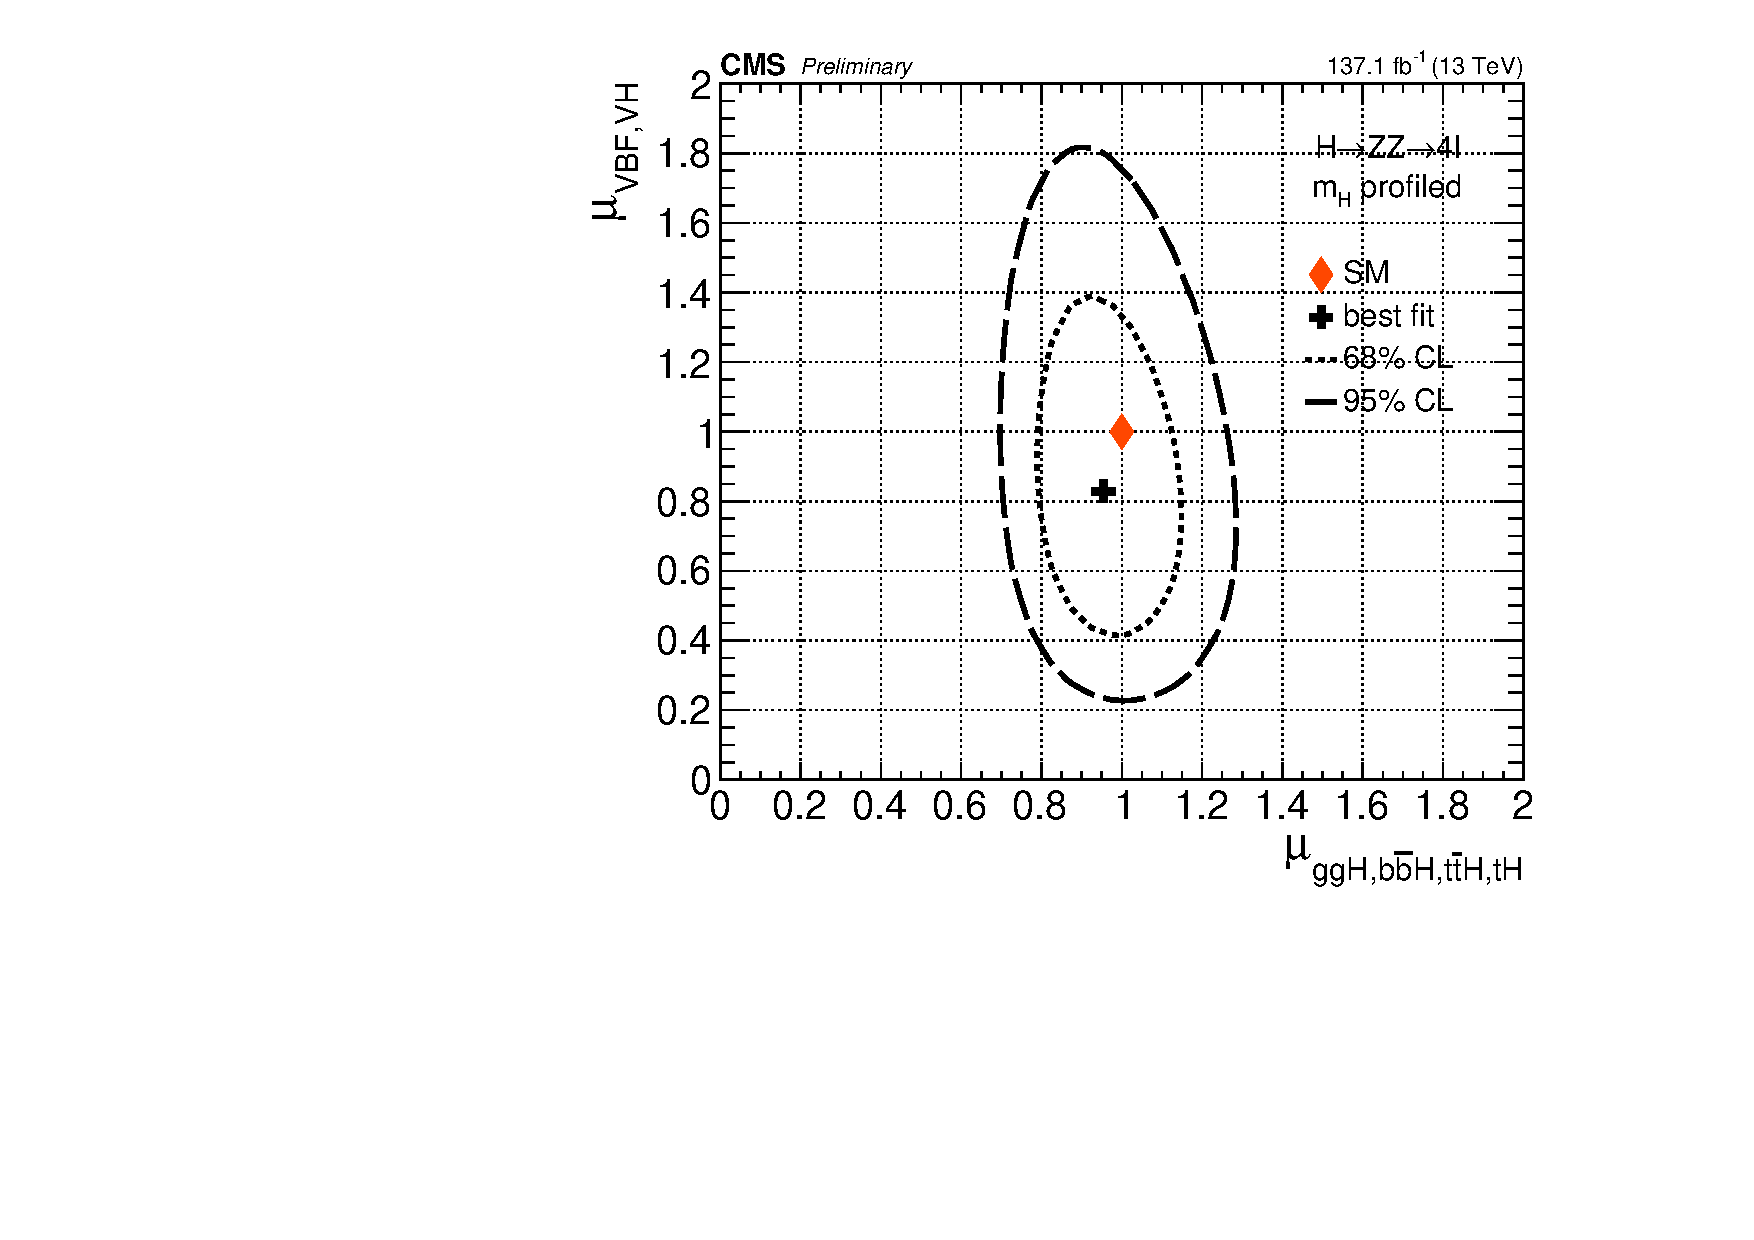
\includegraphics[width=0.6\linewidth]{Figures/results/signalstrength/rvrf.pdf}
    \caption{ Result of the 2D likelihood scan for the $\muF$ and $\muV$ signal-strength modifiers. 
   The solid and dashed contours show the 68\% and 95\% CL regions, respectively. 
    The cross indicates the best-fit values, and the diamond represents the expected values for the SM Higgs boson.
\label{fig:RVRF}}
\end{center}
\end{figure}


%{\renewcommand{\arraystretch}{1.5}
%%%============
%\begin{table}[!hb]
%\begin{center}
%\caption{Expected signal strength values for different measurement setups.
%\label{tab:muvalues_exp}}
%\begin{tabular}{lcccc}
%\hline  
% Categorization  & 1D: ${\cal L}(m_{4l})$ & 2D: ${\cal L}(m_{4l},\KD)$ &   1D: ${\cal L}(m_{4l}')$ & 2D: ${\cal L}(m_{4l}',\KD)$ \\ \hline 
%Inclusive &  $\mu=$1.000$^{+XX}_{-XX}$ & $\mu=$1.000$^{+XX}_{-XX}$ &  $\mu=$1.000$^{+XX}_{-XX}$ & $\mu=$1.000$^{+XX}_{-XX}$ \\ \hline
% &  $\mu=$1.000$^{+XX}_{-XX}$ & $\mu=$1.000$^{+XX}_{-XX}$ &  $\mu=$1.000$^{+XX}_{-XX}$ & $\mu=$1.000$^{+XX}_{-XX}$ \\
%Two categories & $\muV$=1.000$^{+XX}_{-XX}$ & $\muV=$1.000$^{+XX}_{-XX}$ &  $\muV=$1.000$^{+XX}_{-XX}$ & $\muV=$1.000$^{+XX}_{-XX}$ \\
% & $\muF=$1.000$^{+XX}_{-XX}$ & $\muF=$1.000$^{+XX}_{-XX}$ &  $\muF=$1.000$^{+XX}_{-XX}$ & $\muF=$1.000$^{+XX}_{-XX}$ \\
%\hline
%\end{tabular}
%\end{center}
%\end{table}
%%%============
%}
%
%{\renewcommand{\arraystretch}{1.5}
%%%============
%\begin{table}[!hb]
%\begin{center}
%\caption{Expected and observed signal strength values for different measurement setups.
%\label{tab:muvalues_obs}}
%\begin{tabular}{lcccc}
%\hline  
% Categorization  & 1D: ${\cal L}(m_{4l})$ & 2D: ${\cal L}(m_{4l},\KD)$ &   1D: ${\cal L}(m_{4l}')$ & 2D: ${\cal L}(m_{4l}',\KD)$ \\ \hline 
%Inclusive &  $\mu=$X.XX$^{+XX}_{-XX}$ & $\mu=$X.XX$^{+XX}_{-XX}$ &  $\mu=$X.XX$^{+XX}_{-0.XX}$ & $\mu=$X.XX$^{+XX}_{-XX}$ \\ \hline
% &  $\mu=$X.XX$^{+XX}_{-XX}$ & $\mu=$X.XX$^{+XX}_{-XX}$ &  $\mu=$X.XX$^{+XX}_{-XX}$ & $\mu=$X.XX$^{+XX}_{-XX}$ \\
%Two categories & $\muV$=X.XX$^{+XX}_{-XX}$ & $\muV=$X.XX$^{+XX}_{-XX}$ &  $\muV=$X.XX$^{+XX}_{-XX}$ & $\muV=$X.XX$^{+XX}_{-XX}$ \\
% & $\muF=$X.XX$^{+XX}_{-XX}$ & $\muF=$X.XX$^{+XX}_{-XX}$ &  $\muF=$X.XX$^{+XX}_{-XX}$ & $\muF=$X.XX$^{+XX}_{-XX}$ \\
%\hline
%\end{tabular}
%\end{center}
%\end{table}
%%%============
%}

Signal-strength modifiers for the five main Higgs production modes, $\mu_{\Pg\Pg\PH}$, $\mu_{\mathrm{VBF}}$, $\mu_{\WH}$, $\mu_{\ZH}$ and $\mu_{\ttH}$ are also introduced as scale factors to the expected SM cross section. 
Similarly, the fits are performed fixing the mass to $\mH = 125~\GeV$ and profiling the likelihood for all nuisance parameters, leading to the results 
%reported in Table~\ref{tab:muprocesses} and 
illustrated in Fig.~\ref{fig:muprocesses},
% Three models are tested, 
% in Fig.~\ref{fig:muprocesses}(top left) $\mu_{\WH}$ are $\mu_{\ZH}$ are separated, 
% in Fig.~\ref{fig:muprocesses}(top right) $\mu_{\WH}$ are $\mu_{\ZH}$ are grouped in $\mu_{\VH}$, 
% and in Fig.~\ref{fig:muprocesses}(bottom) 
where $\mu_{\WH}$ and  $\mu_{\ZH}$ are merged to $\mu_{VH}$.
%splitted in the leptonically decay bosons  $\mu_{\WH lep}$/$\mu_{\ZH lep}$ and hadronically decay  bosons $\mu_{\WH lep}$/$\mu_{\ZH lep}$.


%%%============
%\begin{table}[hb]
%\begin{center}
%\caption{Expected and observed results of likelihood scans for the signal strength modifiers corresponding to the five main Higgs boson production modes.
%\label{tab:muprocesses}}
%\begin{tabular}{l|c|c}
%\hline
%   & Expected & Observed  \\
%\hline
%$\mu_{\Pg\Pg\PH}$  & 1.00$^{+0.48}_{-0.43}$ & 1.09$^{+0.47}_{-0.42}$  \\
%$\mu_{\mathrm{VBF}}$  & 1.00$^{+2.51}_{-1.00}$ & 0.00$^{+0.59}_{-0.00}$  \\
%$\mu_{\WH}$  & 1.00$^{+9.20}_{-1.00}$ & 0.00$^{+8.49}_{0.00}$  \\
%$\mu_{\ZH}$  & 1.00$^{+17.96}_{-1.00}$ & 2.48$^{+17.43}_{-2.48}$  \\
%$\mu_{\ttH}$  & 1.00$^{+8.01}_{-1.00}$ & 8.83$^{+16.39}_{-8.83}$ \\
%\hline
%\end{tabular}
%\end{center}
%\end{table}
%%%============

\begin{figure}[htb]
\begin{center}
% \includegraphics[width=0.45\linewidth]{Figures/Results/signalstrength/compatibility_process_ZHWH.pdf}
% \includegraphics[width=0.45\linewidth]{Figures/Results/signalstrength/compatibility_process_VH.pdf} \\
%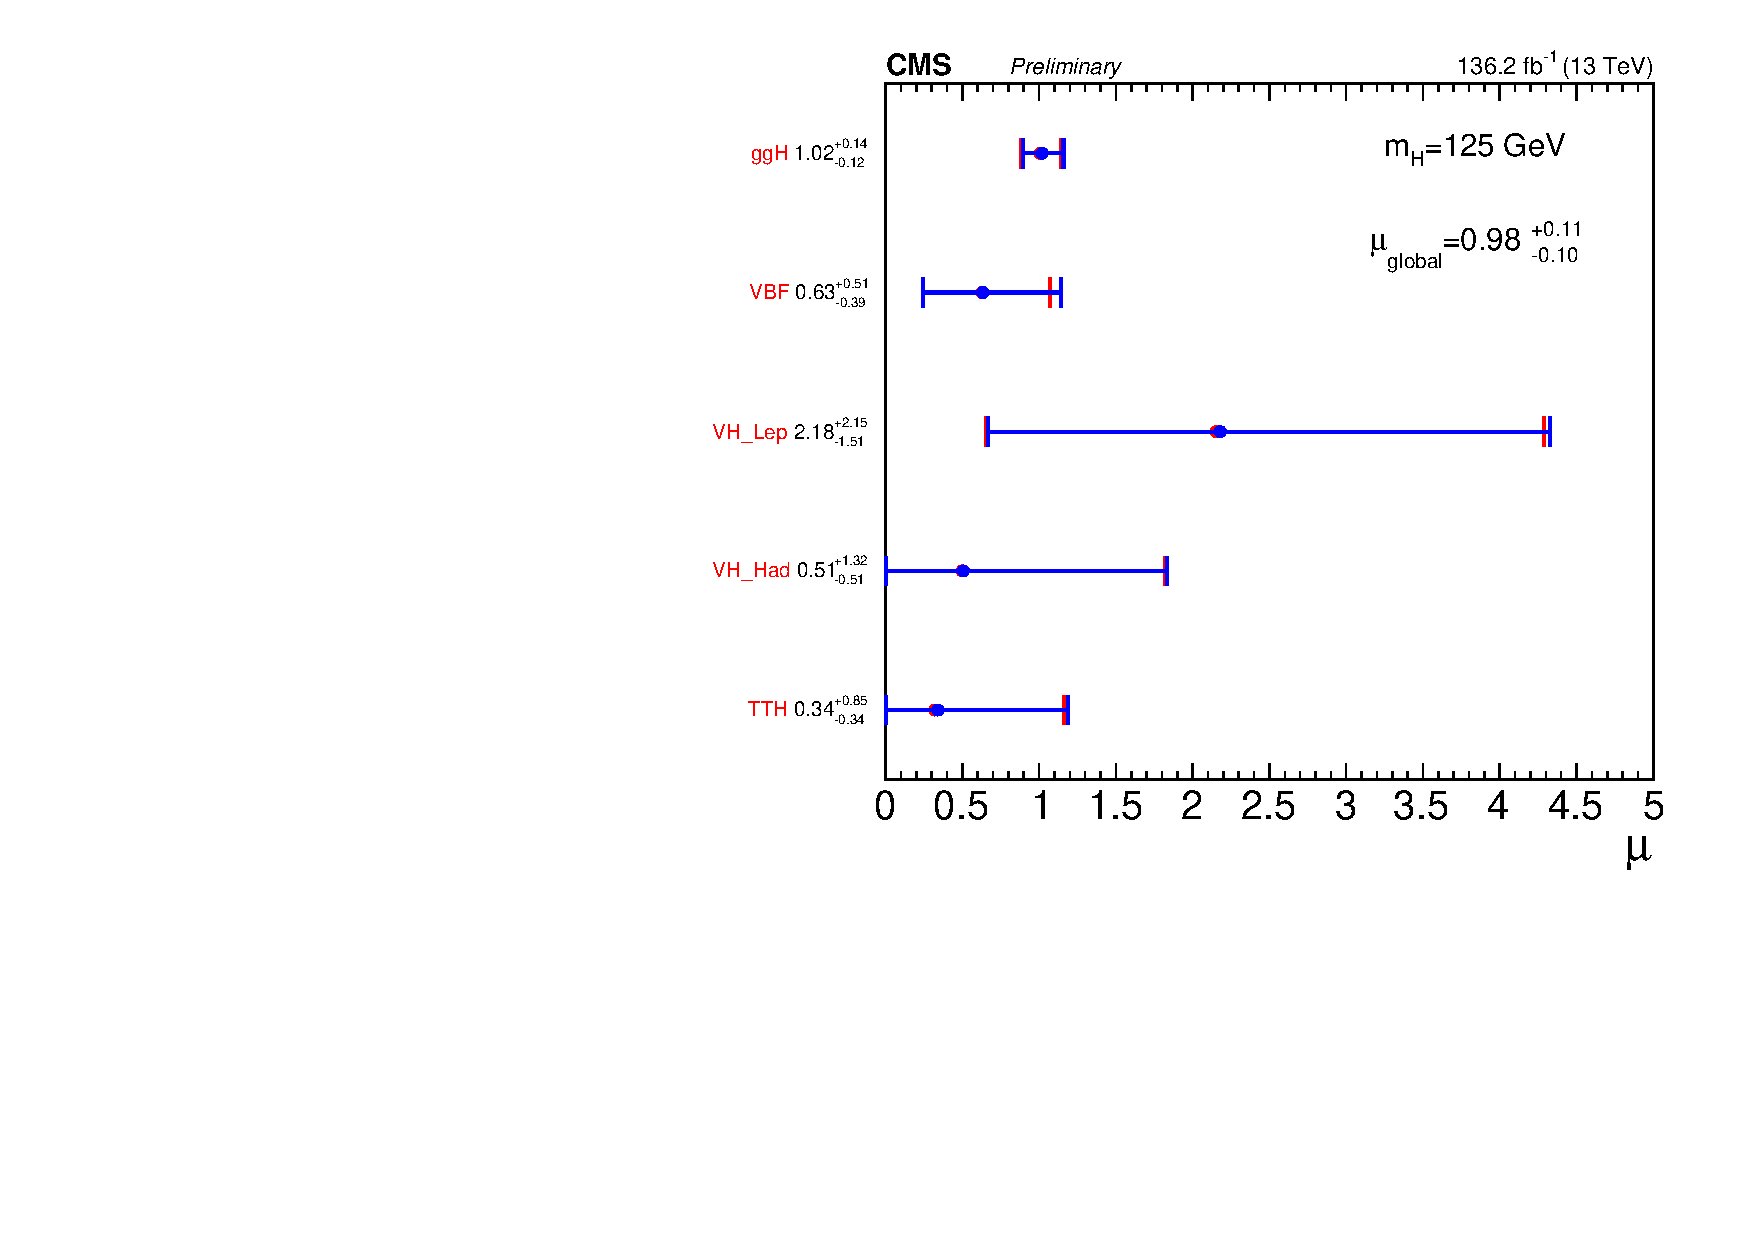
\includegraphics[width=0.80\linewidth]{Figures/results/signalstrength/mu_stage0_hadlep1_obs.pdf}
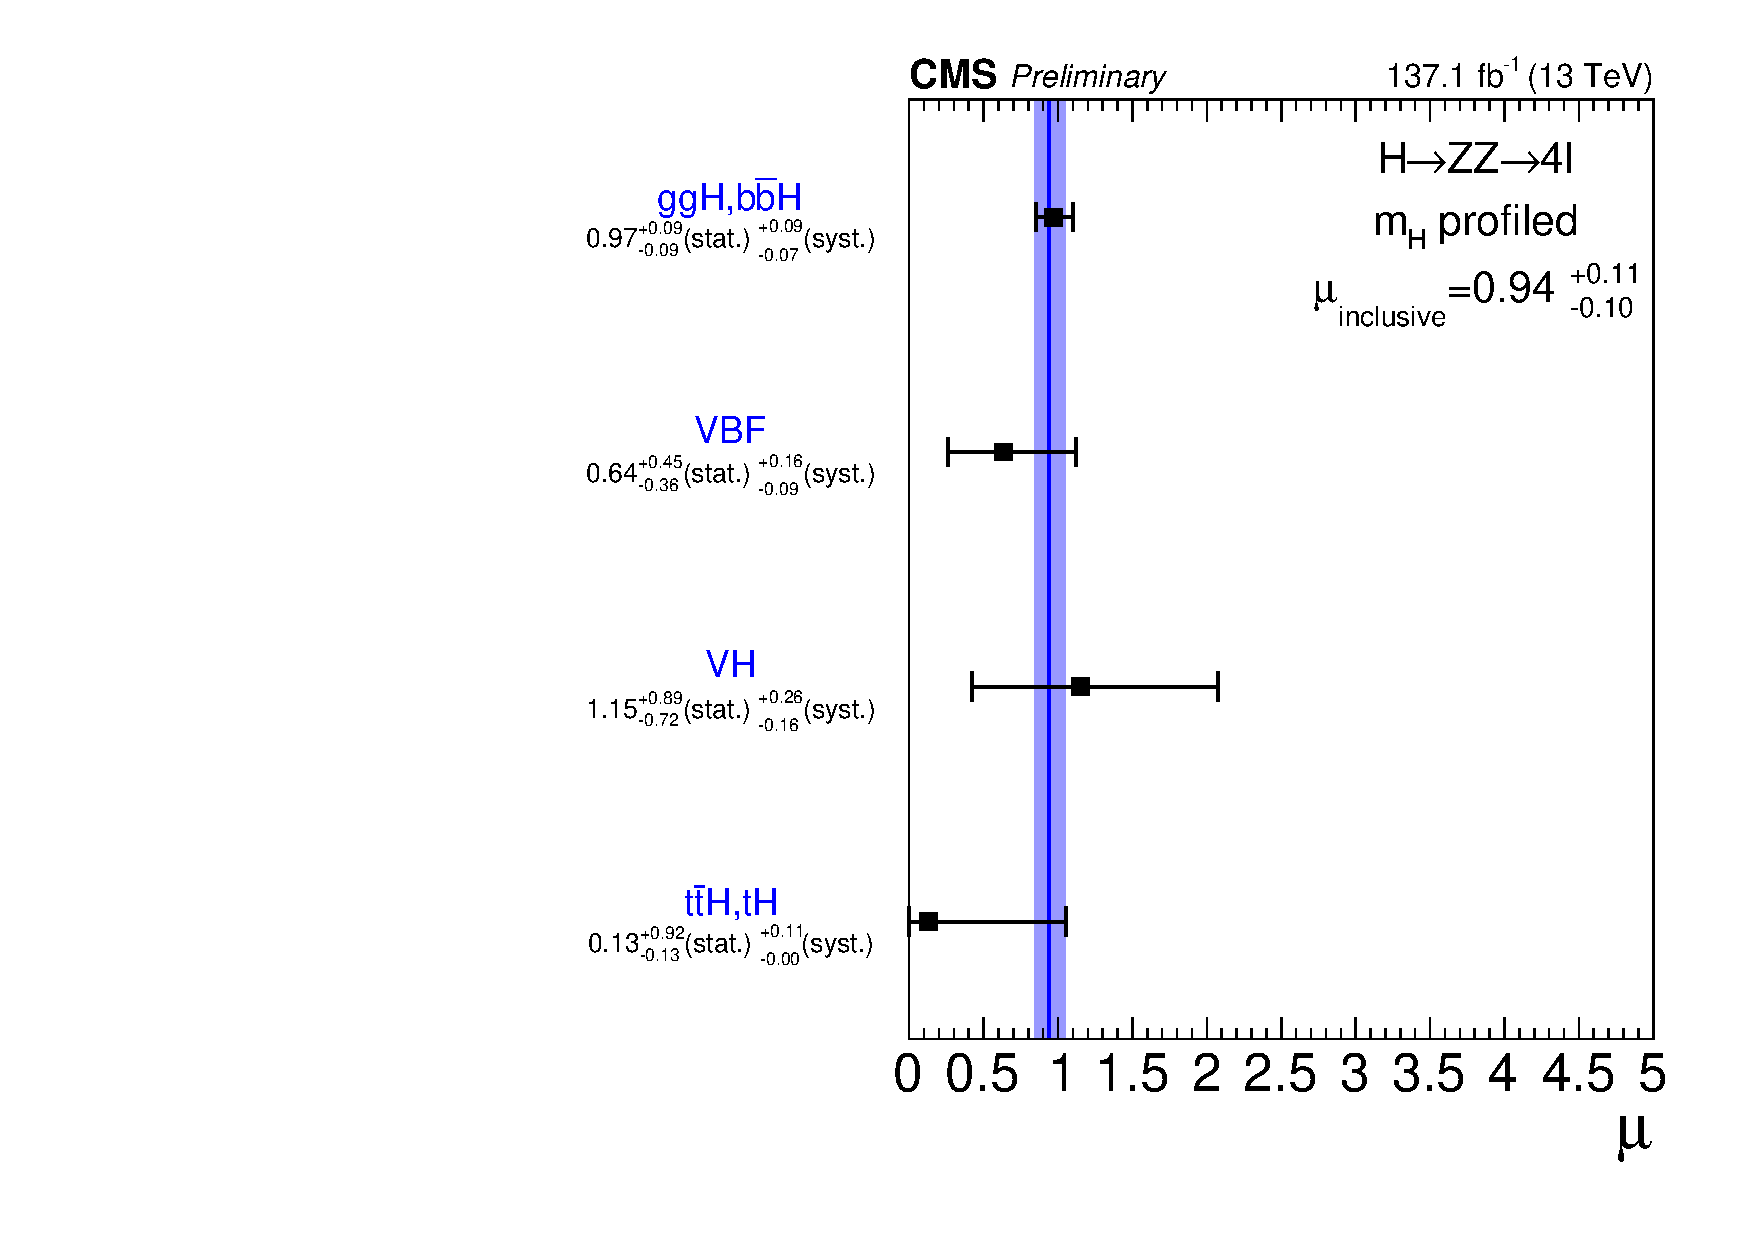
\includegraphics[width=0.45\linewidth]{Figures/results/signalstrength/mu_stage0.pdf}
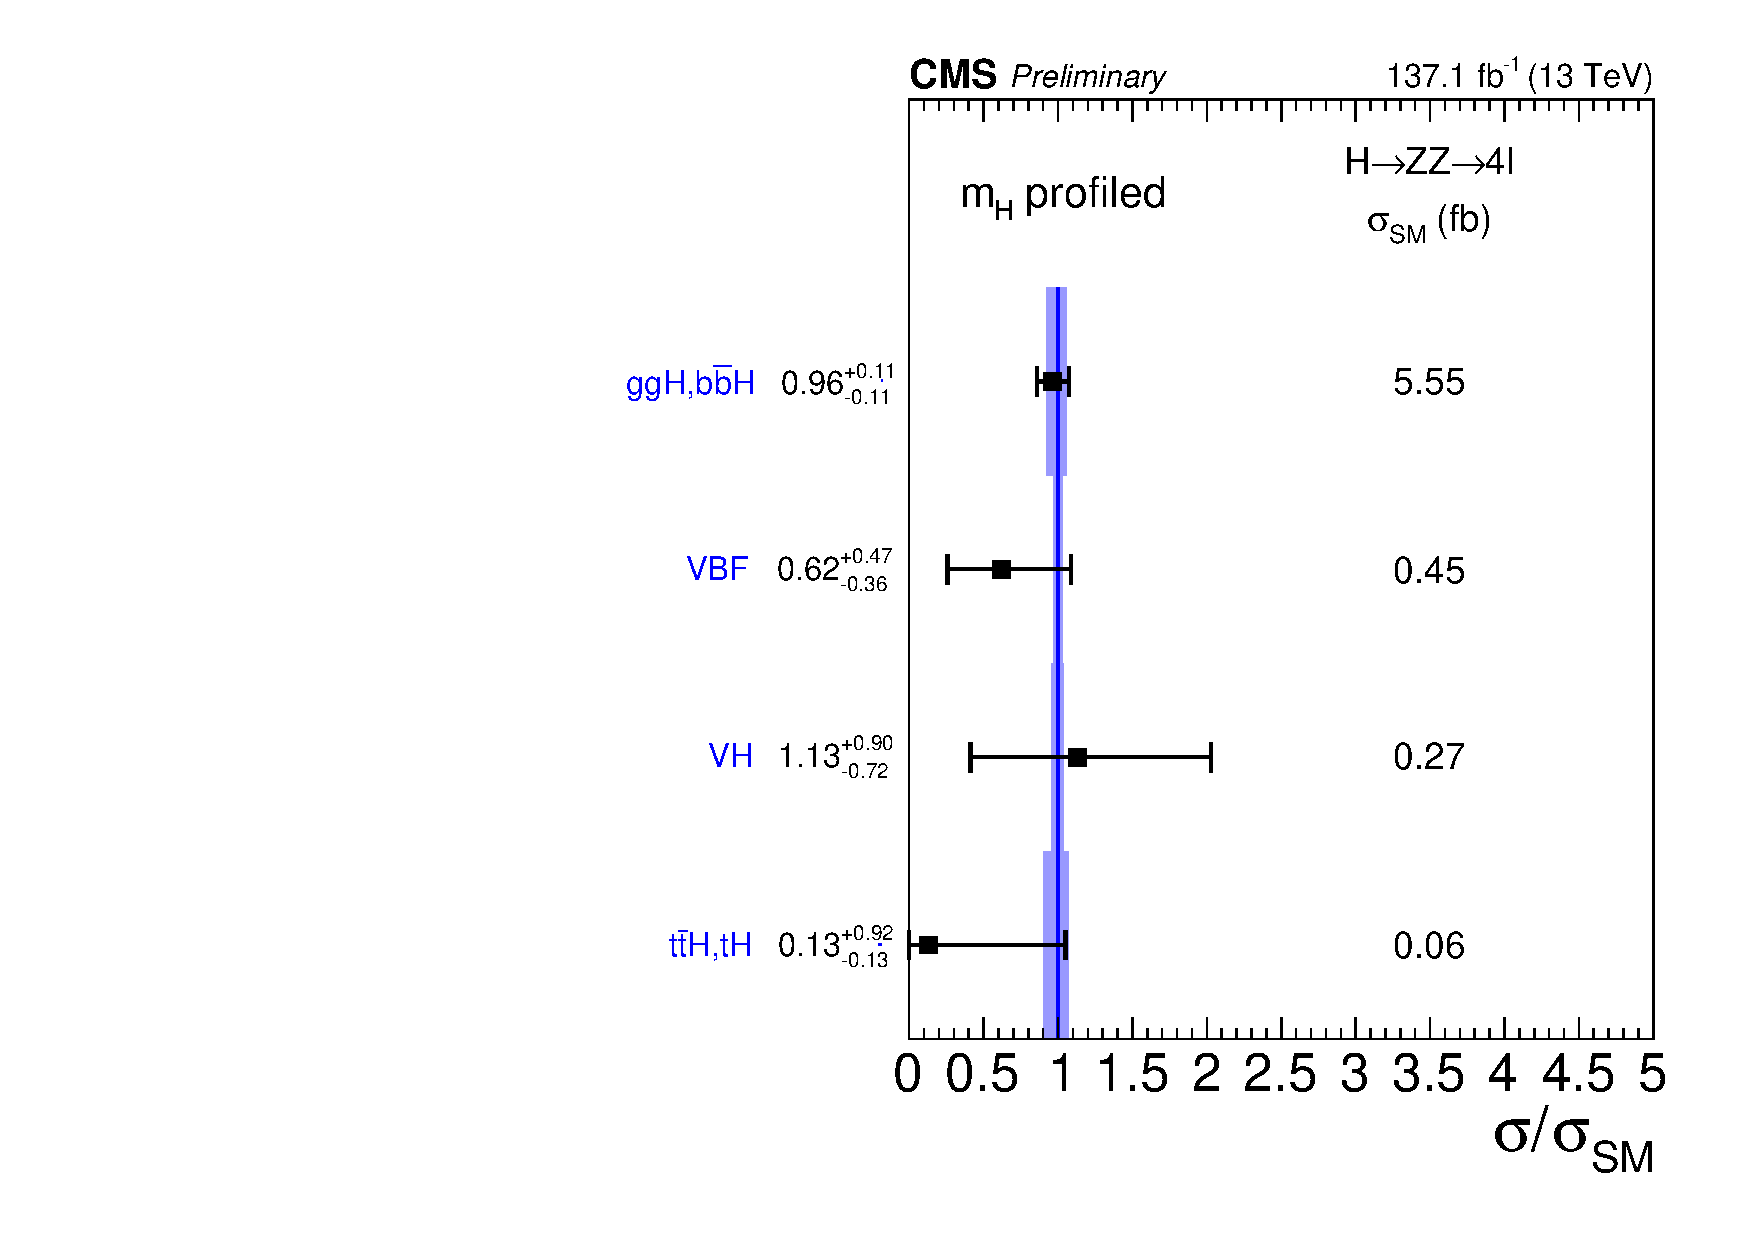
\includegraphics[width=0.45\linewidth]{Figures/results/signalstrength/mu_stage0_xsec.pdf}
\caption{Results of likelihood scans for the signal strength modifiers (left) and cross section (right) corresponding to the four main Higgs boson production modes.
On the left figure, the vertical line shows the combined $\mu$, together with its associated $\pm$ 1$\sigma$ uncertainties shown as filled band.  
On the right figure, the band of the vertical line shows the theoretical uncertainties on the SM cross sections.
The horizontal bars indicate the $\pm$ 1$\sigma$ uncertainties on $\mu$ for the different production modes. 
The uncertainties include both statistical and systematic sources.
\label{fig:muprocesses}}
\end{center}
\end{figure}
